\chapter{Introdução}
A mortalidade infantil é um problema social que ocorre em escala global e a redução
dela faz parte das Metas do Desenvolvimento do Milênio, compromisso assumido pelos países
integrantes da Organização das Nações Unidas (ONU), do qual o Brasil é signatário.

A taxa de mortalidade infantil consiste na relação entre o óbito de crianças no primeiro ano
de vida e a quantidade de nascidos vivos do mesmo período. Para facilidade de comparação entre
os diferentes países ou regiões do globo esta taxa é normalmente expressa em número de óbitos a
cada mil nascidos vivos.

No Brasil tem sido observado um declínio nesta taxa, como pode-se observar no gráfico a seguir:

\begin{center}
\begin{figure}[h]
  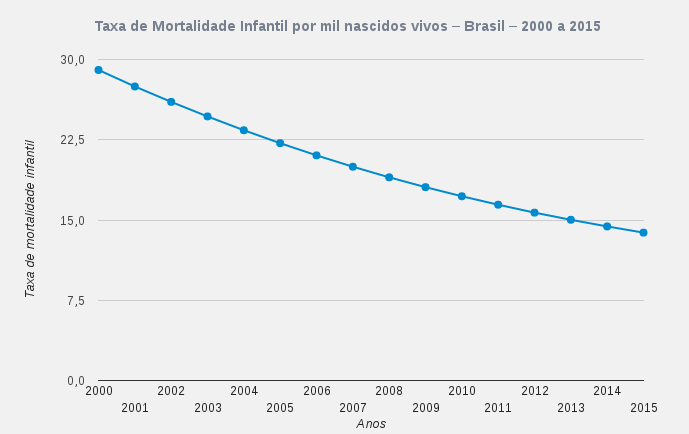
\includegraphics[width=\linewidth]{mortalidade_infantil.png}
\end{figure}
Fonte: \cite{ibgeMortalidade}
\end{center}

Apesar da significativa redução através dos anos, o Brasil ainda precisa melhorar
muito em relação aos países de primeiro mundo. A taxa de mortalidade atual (13,82/1000 nascidos vivos)
é cerca de três a seis vezes maior que a de países desenvolvidos, como Japão, Canadá e Alemanha que
apresentam taxa de 3 a 10/1000 nascidos vivos.

Numa situação ideal, esperaria-se que nenhuma criança morresse no primeiro ano de vida; nas situações
reais, é impossível reduzir a taxa de mortalidade infantil a zero, pois algumas crianças nascem com doenças
tão graves que a atual tecnologia médica disponível ainda não pode salvar suas vidas (ex: anencefalia).

Entretanto, a maioria das mortes precoces podem ser evitadas com o fácil e rápido acesso a serviços qualificados de saúde
e com a prevenção de doenças conhecidas. Além disso, fatores externos também
contribuem para a mudança desta taxa, como acesso ao  saneamento básico, taxa de fecundidade,
segurança alimentar e nutricional, grau de instrução das mulheres, avanço das tecnologias médicas,
em especial a imunização e terapia de reidratação oral, prevalência do aleitamento materno,
entre outros \cite{lansky2009mortalidade}, \cite{frias2008politicas}.

Para entender melhor a dinâmica da taxa de mortalidade infantil, estudar como cada um destes elementos
afeta a mesma torna-se uma necessidade.

A associação entre saneamento e saúde já foi objeto de inúmeros estudos \cite{libanio2005dimensao},
\cite{teixeira2011analise}, \cite{costa2002indicadores} e é consenso a afirmação de que o saneamento
básico afeta diretamente na qualidade de vida e mortalidade da população. Isso se explica pelas doenças
que são transmitidas em decorrência deste fato que afeta principalmente crianças e idosos
\cite{libanio2005dimensao}.

No âmbito do saneamento, dois fatores se destacam: A cobertura por esgotamento sanitário e a cobertura
por serviços de coleta de lixo. \cite{teixeira2011analise} diz que a baixa cobertura por esgotamento sanitário
nos estados brasileiros contribui para a mortalidade infantil no país. \cite{libanio2005dimensao} constata que a condição de vida das
populações é retratada pela abrangência dos serviços de água e esgoto e lixo.

Devido às evidências apresentadas, escolhemos fazer um estudo de regressão linear múltipla utilizando a
taxa de mortalidade infantil como variável dependente, e como variáveis independentes utilizamos a proporção
da população servida por esgotamento sanitário (dado em \%) e a proporção da população servida por coleta de
lixo (dado em \%).

Os dados utilizados foram retirados do site do IDB \cite{idb}, plataforma oficial do Ministério da Saúde para
assuntos relacionados.

Foram utilizados dois softwares para o processamento de dados estatísticos: Excel 2015 e o software R
através de sua plataforma web \cite{wessa}. O seguinte trabalho está estruturado da seguinte forma: seção 2.
Desenvolvimento da Regressão Linear. seção 3. Validação do modelo proposto, seção 4. Conclusão e seção 5
Referências Bibliográficas.
